\chapter{Organisations Secrètes ou Non}

\begin{multicols*}{2}

\section{Le Conseil Galactique Criminel}

Lors de la domination Ergios, chaque peuple possédait ses propres réseaux criminels bien diversifiés. Ceux-ci agissaient prudemment, dans l’ombre, les lois Ergios étant particulièrement difficiles et les forces de polices Ergios performantes. Lors de la guerre d’indépendance, les différents groupuscules criminels ont décidé de tirer leur épingle du jeu et de se réorganiser sérieusement, de se regrouper.

Le Conseil Galactique Criminel a alors été fondé. Ce conseil n'est pas une alliance ou une pègre unique, il s'agit d'un ensemble de règles et d'accords permettant de réguler l'activité criminelle et d'éviter les débordements. Le Conseil n'évite pas, par exemple, les conflits de frontières entre deux pègres. Il les réglemente toutefois pour que le conflit évite de nuire trop aux profits, et évite également d'attirer trop l'attention des autorités qui pourraient alors prendre des mesures trop brutales.

\parpic[l]{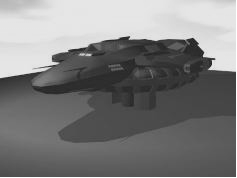
\includegraphics[width=120pt]{image/vaisseau2.png}}  Une fois la guerre terminée, les pègres et associations de malfaiteurs étaient trop fortement implantés dans la société pour que la renaissante Fédération Galactique puisse s’y opposer. La nouvelle explosion des conflits n'a fait que renforcer les pouvoirs de la pègre, principalement en dehors des grandes capitales ou la pègre est presque devenue maître de l'organisation judiciaire...

\section{Snag'Norak}

On oublie souvent les Snagirs à cause de leur aspect inoffensif et de leur grande discrétion dans les affaires sociales, et pourtant la Snag’Norak est une pègre qui n’est pas à négliger. Elle possède des moyens technologiques très avancés pour atteindre leur but !

Officiellement, la Snag’Norak peut accueillir des non Snagirs, officieusement les quelques cas existants sont isolés. L’organisation de la Snag’Norak est très proche de l’organisation de leur pays. Des rumeurs disent que la Snag’Norak contrôle le marché noir du Sagium.

Pour différentes raisons, la Snag'Norak a refusé de signer les accords du CGC. Toutefois il y a très peu de conflit entre les deux forces : la Snag'Norak est le maître incontesté en territoire Snagir et ne cherche que très peu à s'étendre en dehors.

\section{Antalgis}

Certains voit l'Antalgis comme un groupe criminel qu'il faut abattre à tout prix, d'autres les perçoivent comme des gardiens de la liberté, des guerriers prêts à sacrifier leur vie pour leur cause, des héros... L'Antalgis est un groupe luttant pour la fin de l'esclavagisme dans les mondes connus et donc, la libération de tous les Teldrims Esclaves.

Leurs actions visent principalement cette libération, ou l'atteinte des infrastructures, des gouvernements ou des corporations favorisant et abusant de l'esclavagisme. Ceux-ci prennent d'ailleurs la menace de l'Antalgis très au sérieux car ce groupe a déjà montré maintes fois sa détermination.

En plus de ces membres, l'Antalgis est soutenue par de nombreux sympathisants, qui sans participer activement à la lutte, sont prêts à collaborer en leur fournissant de nombreux renseignements.

Le gouvernement Teldrim mène une lutte acharnée contre l'Antalgis partout dans les mondes connus. Les rumeurs racontent que l'Alliance Terrienne fournirait à l'Antalgis des armes, ce qui n'est pas pour arranger les relations entre les deux gouvernements.

\section{Aube pourpre}

L'aube pourpre est une secte qui inquiète beaucoup les autorités. Elle considère les Ergios comme des dieux. Pour ses membres, les gouvernements raciaux sont responsables de l'hérésie qui a chassé les dieux et doivent absolument être détruits.

Ils sont prêts à tout pour atteindre leur but. L'Aube Poupre est constituée d'extrêmistes prêts à sacrifier leur vie pour leur objectif. Ils ont sombré dans un terrorisme violent, entraînant dans leurs actions un grand nombre de civils. Ils considèrent également les Eskadors comme une punition divine.

\end{multicols*}
